\chapter{Markov链与模型}\label{chap:markov-chain}

我们都知道,人的推理和决策会受到时间的影响:我们宁愿要现在的十块钱也不要十年后的二十块钱. 然而,人和人的耐心程度是不一样的. 2010年,来自意大利博洛尼亚大学Manuela Sellitto和她的同事进行了一项实验. 他们的实验对象是一组大脑正常的人(对照组)、一组非眶额叶区受损的病人(实验组1)和一组眶额叶周围受损的病人(实验组2). 实验人员对被试进行提问,典型的问题如下:“你想要现在拿到10美元还是一个月后拿到12美元?”. 他们对食物和货币形式的奖励都进行了测试. 

结果显示,眶额叶周围受损的病人更倾向于选择即时的奖励,而其他组的人更倾向于选择未来的奖励. 如果货币奖励翻倍(例如,从50美元变为100美元),对照组和实验组1的人愿意等待4到6个月,而眶额叶周围受损的人(实验组2)甚至不愿意等待3周. 换句话说,人的耐心程度是大脑结构决定的,而不是自己可以轻易改变的!

以上例子不仅说明时间在决策中的重要性,更说明人脑中有特殊的结构和机制处理时间相关的决策问题. 这样的观察对于人工智能也是同样重要的. 本章我们将介绍Markov链,这是一种带有时间的概率模型,它是应用最为成功的含时决策模型之一. 我们还将介绍人工智能领域基于Markov链的各种应用,包括Markov决策模型与强化学习、隐Markov模型以及扩散模型. 

\section{Markov链}

在\Cref{chap:plausible-reasoning}中,我们说明了合情推理是人和AI非常重要的推理方式,这一推理模式基于Bayes概率论和似然. 然而,这一模型对推理的假设是逻辑的、静态的,时间的概念并不出现在似然里面. 例如,考虑一个罐子,里面有除颜色之外不可区分的$N$个球,有$n$个白球,剩下的是黑球. 顺序从中拿出$N$个球,第$k$次拿出的球颜色是$W_k$或$B_k$.

用Bayes定理很容易证明,对任意$i\neq j$,$\Pr(W_i|W_j)=\Pr(W_j|W_i)$. 也就是说,$\Pr(W_i|W_j)$和$\Pr(W_j|W_i)$不仅是可计算的,而且是相等的. 然而,如果从推理的角度来说,我们基于时间更晚的状态推理时间更早的状态,这样的推理需要我们能够有对未来的模型. 因此,我们需要引入一个带有时间的推理模型,这就是Markov链.

\begin{definition}[Markov链]
\textbf{Markov链}(\textbf{马氏链})是一列随机变量$\{X_t\}_{t=0}^{\infty}$,包含如下概念:
\begin{itemize}
	\item \emph{状态空间} $\calS$:$X_t$所有可能值构成的集合,有限或者可数.
	\item \emph{转移矩阵} $\calP$(\emph{转移核}):下一时刻系统状态之间转移的概率. $\calP=(p_{ij})_{i,j\in \calS}$,$p_{ij}$是从$i$状态转移到$j$状态的概率.
	\item \emph{Markov性}: 对任意时刻$t=1,\dots,n$和任意状态$j,k,j_0,\dots,j_{t-1}\in \calS$,如下等式成立
		\begin{align*}
		   &\Pr(X_{t+1}=j| X_t=k,X_{t-1}=j_{t-1},\dots,X_0=j_0)\\
           =&\Pr(X_{t+1}=j| X_{t}=k)=p_{kj}.
		\end{align*}
    \end{itemize}
    有时候也考虑带初态的Markov链,此时$X_0$服从分布$\lambda=(\lambda_s)_{s\in \calS}$.
\end{definition}
我们给出的定义是简化的Markov链,每个时刻之间的转移都是一样的转移矩阵,这样的Markov链被称为\emph{时齐的}. 有时候也会考虑非时齐的Markov链(例如扩散模型),即每个时刻之间的转移矩阵不一样,这样的Markov链被称为\emph{非时齐的},此时$t$时刻的转移矩阵是$\calP^{(t)}$,定义中Markov性的转移概率是$p_{kj}^{(t)}$.

Markov链是一种简化的带时间的概率模型,它最重要的性质是Markov性,即在固定现在的情况下,过去与未来相互独立. 这一性质的数学表述为:
\begin{proposition}[Markov性]\label{prop:markov}
条件在$X_n=i$下,$\{Y_m\}_{m=0}^{\infty}:=\{X_{m+n}\}_{m=0}^{\infty}$是一个转移矩阵为$P$的Markov链,并且与$(X_0,\dots,X_{n-1})$相互独立. % HW: 证明这个命题
\end{proposition}
证明留做习题. 

我们考虑的Markov链还有时齐性,即状态的转移不依赖当前时间,只和当前的状态有关. 时齐性的数学表述为:
\begin{proposition}
    设$\{X_t\}_{t=0}^{\infty}$是一个Markov链,那么对任意的$t,m,n\in \N$和$i,j,k\in \calS$,有
    $\Pr(X_{m+n}=j| X_{n}=k)=\Pr(X_{m}=j| X_{0}=k)$.
\end{proposition}

我们来看一个Markov链的例子. 
\begin{example}[赌徒模型]
    考虑公平对赌. 玩家$A$和$B$抛硬币来赌钱,$A$赌正面,$B$赌反面. 每一轮独立地抛硬币,正面朝上的概率和反面朝上的概率相等,都是$1/2$. 赢的一方给输的一方一块钱. $A$输$a$块钱破产,$B$输$b$块钱破产,$Z_i$是第$i$轮$A$的收入. $Z_0=X_0=0$是$A$初始的收入. $X_n=Z_0+\dots+Z_n$是$A$的累计收入. 那么,$\{X_n\}_{n\geq 0}$是一个Markov链.
    \begin{itemize}
        \item 状态空间:$\calS=\{-a,-a+1,\dots,0,1,\dots,b\}$.
        \item 转移概率:对$-a<i<b-1$,$p_{i,i+1}=p_{i+1,i}=1/2$;$p_{-a+1,-a}=p_{b-1,b}=1/2$,$p_{-a,-a}=p_{b,b}=1$;其他值为$0$.
    \end{itemize}
    转移矩阵可以画成\Cref{fig:gambling} 所示的形式.
    \begin{figure}[H]
    \centering
    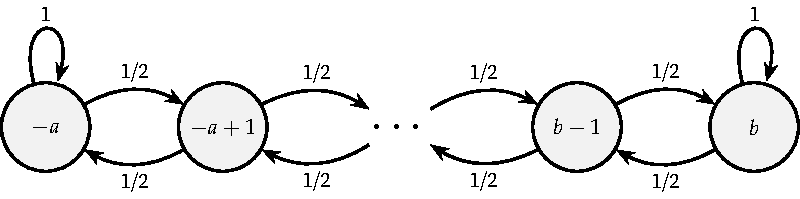
\includegraphics[width=0.9\textwidth]{figures/Markov-chain/gampling.pdf}
    \caption{赌徒模型的转移矩阵}\label{fig:gambling}
    \end{figure}
    一般地,任何时齐可数状态的Markov链都可以用图表示.
\end{example}

接下来,我们来看一个非时齐的Markov链的例子.

\begin{example}[Pólya的坛子]
想象现在有一个坛子. 开始的时候,坛子里有$1$个白球和$1$个黑球. 每一轮,我们从坛子里随机拿出一个球,观察颜色,然后放回去,再加入一个和刚才拿出的球颜色相同的球. 例如,如果第一轮我们拿出一个白球,那么第二轮开始时坛子里有$2$个白球和$1$个黑球. 

设$X_t$是第$t$轮之后白球的数量,我们会发现,它是一个非时齐的Markov链,转移概率为
\begin{itemize}
    \item $\Pr(X_{t+1}=i+1|X_t=i)=i/(t+2)$,
    \item $\Pr(X_{t+1}=i|X_t=i)=(t+1-i)/(t+2)$,
    \item 其他值的概率为$0$. 
\end{itemize}
这个Markov链的一个重要性质是当$t\to\infty$时,$X_t/t$趋于均匀分布$\U[0,1]$. 

这个性质可以通过对$t$进行归纳证明,即$X_t$是$\{1,\dots,t+1\}$上的均匀分布. $t=0$时,$X_0=1$,显然成立. 假设对$t$成立,即$X_t$是$\{1,\dots,t+1\}$上的均匀分布. 那么对$t+1$以及$1\leq j\leq t+2$,根据全概率公式,我们有
\begin{align*}
    \Pr(X_{t+1}=j)&=\sum_{k=1}^{t+1}\Pr(X_{t+1}=j|X_t=k)\Pr(X_t=k)\\
    &=\frac{1}{t+1}(\Pr(X_{t+1}=j|X_t=j-1)+\Pr(X_{t+1}=j|X_t=j))\\
    &=\frac{1}{t+1}\left(\frac{j-1}{t+2}+\frac{t+2-j}{t+2}\right)=\frac{1}{t+2}.
\end{align*}
于是,归纳成立.

Pólya的坛子还有一种有趣的解读:如果我们把人生的每一次选择都看成放球,我们经常会基于现在看到的东西(看到的黑球还是白球)投资自己的人生(放一个黑球还是白球),这样的结果是我们的人生会多姿多彩,百花齐放. 
\end{example}

我们回到赌徒模型. $A$的累计收入$\{X_n\}_{n\geq 0}$形成了Markov链. 根据Markov性,未来双方的收入变化只取决于现在,而和过去运气无关. 与之相关的一个现象是赌徒谬误,即认为过去的运气会影响未来的运气. 例如,如果一个人连续输了很多次,那么他会认为自己未来运气会变好,赢的概率更大. 但是,根据Markov性,过去的运气不会影响未来的运气,因此这种想法是错误的. ``风水轮流转''在一场公平对赌中是不正确的认知. 那么,如何评估赌局的公平性?

如果对赌是公平的,那么我们应该认为两个人每一轮的累计收入分布都是一样的,即
    \[\Pr(X_n=i|X_0=0)=\Pr(X_n=-i|X_0=0).\]
因此,我们需要能够计算多步转移的概率. 设$p_{ij}^{(k)}$表示从状态$i$用$k$步转移到状态$j$的概率. $k$步转移概率形成了一个矩阵$\calP^{(k)}$. 下面的定理给出了计算\emph{多步转移概率}的方法.

\begin{theorem}[Kolmogorov-Chapman方程]\label{thm:kolmogorov-chapman}
    $P^{(k+l)}=\calP^{(k)}\calP^{(l)}$.
\end{theorem}

\begin{proof}
由Markov性、时齐性和全概率公式,
\begin{align*}
    p_{ij}^{(k+l)} &= \Pr(X_{k+l}=j|X_0=i) \\
 &= \sum_{\alpha}\Pr(X_{k+l}=j,X_k=\alpha|X_0=i) \\
 &= \sum_{\alpha}\Pr(X_k=\alpha|X_0=i)\Pr(X_{k+l}=j|X_k=\alpha) \\
 &= \sum_{\alpha} p_{i\alpha}^{(k)}p_{\alpha j}^{(l)}.
\end{align*}
\end{proof}

Kolmogorov-Chapman方程有两个重要的特例,前向方程:
\[\calP^{(k+1)}=\calP^{(k)}\calP,\]
以及后向方程:
\[\calP^{(l+1)}=\calP\calP^{(l)}.\]
这一过程示意见\Cref{fig:forward-equation} 和\Cref{fig:backward-equation}.
\begin{figure}[ht]
    \begin{minipage}[t]{0.45\linewidth}
        \centering
        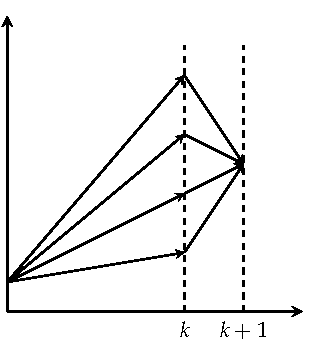
\includegraphics[width=0.8\linewidth]{figures/Markov-chain/forward-equation.pdf}
        \caption{前向方程(往前一步)}
        \label{fig:forward-equation}
    \end{minipage}
    \hfill
    \begin{minipage}[t]{0.45\linewidth}
        \centering
        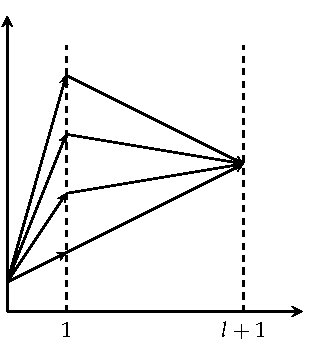
\includegraphics[width=0.8\linewidth]{figures/Markov-chain/backward-equation.pdf}
        \caption{后向方程(往回一步)}
        \label{fig:backward-equation}
    \end{minipage}
\end{figure}

此外,利用归纳法,我们还有如下推论:
\begin{corollary}\label{cor:kolmogorov-chapman}
    $\calP^{(k)}=\calP^k$.    
\end{corollary}

若已知初始分布向量为$\lambda$,利用这一推论,我们可以计算它随时间的演化:
	\[\lambda^\t,\lambda^\t \calP,\dots,\lambda^\t \calP^n,\dots\] %HW: 证明这个演化

回到赌徒模型,如何计算公平对赌中$X_n$的概率分布?我们先来看一个简化的例子. 考虑只有两个状态$0,1$,转移矩阵为
	\[\calP=\begin{pmatrix}p_{00}&p_{01}\\p_{10}&p_{11}
	\end{pmatrix}.\]
或者画成\Cref{fig:simple-example} 的形式.
\begin{figure}
    \centering
    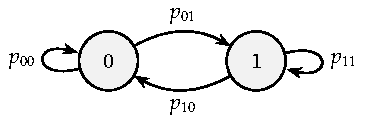
\includegraphics[width=0.5\textwidth]{figures/Markov-chain/simple-example.pdf}
    \caption{只有两个状态的Markov链}
    \label{fig:simple-example}
\end{figure}

可以归纳证明:
\begin{align*}
    \calP^n=&\frac{1}{2-p_{00}-p_{11}}\begin{pmatrix}1-p_{11}&1-p_{00}\\1-p_{11}&1-p_{00}\end{pmatrix}\\
    &+\frac{(p_{00}+p_{11}-1)^n}{2-p_{00}-p_{11}}\begin{pmatrix}1-p_{00}&-(1-p_{00})\\-(1-p_{11})&1-p_{11}\end{pmatrix}.
\end{align*}
假设$|p_{00}+p_{11}-1|<1$,等价地,$p_{00}$和$p_{11}$不同时为$0$或同时为$1$,那么
    \begin{itemize}
        \item $\lim_{n\to\infty}p_{i0}^{(n)}=(1-p_{11})/(2-p_{00}-p_{11})$,
        \item $\lim_{n\to\infty}p_{i1}^{(n)}=(1-p_{00})/(2-p_{00}-p_{11})$.
    \end{itemize}
因此,无论初始分布是什么,随着时间的推移,Markov链的分布会收敛到一个同一个稳定的分布. 这个例子是否具有普遍性?

我们再考虑一个例子. 一个四元环$\Z_6=\{0,1,2,3\}$上的Markov链$X_k$,转移矩阵为$p(i,i+1)=p(i,i-1)=1/2$,这里的表达式将$-1$和$4$等同,$4$和$0$等同. 如果初始分布集中在$0$上,那么我们会发现以概率$1$有$X_{2k}\in\{0,2\}$,$X_{2k+1}\in\{1,3\}$. 这种情况下,最终不会趋于一个稳定的分布!如果初始分布等概率地分布在$\{0,1\}$上,最终会趋于一个$\Z_4$上的均匀分布. 因此,并不是所有Markov链都具有这样的性质. 然而, 对于相当广泛的一类Markov链,这一结论成立,这就是\emph{遍历定理}.

\begin{theorem}[遍历定理]\label{thm:ergodic-theorem}
    设Markov链的状态空间为$\calS=\{1,\dots,N\}$,转移矩阵为$\calP=(p_{ij})$. 如果存在某个$n_0$,使得
    \begin{equation}
        \min_{ij}p_{ij}^{(n_0)}>0,\label{eq:reachable}
    \end{equation}
    那么存在分布$\lambda=(\lambda_1,\dots,\lambda_N)$使得
    \begin{equation}
        \lambda_i>0,\quad\sum_i\lambda_i=1,\label{eq:positive-distribution}
    \end{equation}
    并且对于每一个$j\in\calS$和任意$i\in\calS$都有
    \begin{equation}
    p_{ij}^{(n)}\to\lambda_j,n\to\infty.\label{eq:converge-to-limit}
    \end{equation}
    反之,如果存在满足 \eqref{eq:positive-distribution} 和 \eqref{eq:converge-to-limit} 的$\lambda$,则存在满足 \eqref{eq:reachable} 的$n_0$.

    最后,在以上条件下,\eqref{eq:positive-distribution} 的$\lambda$满足
    \begin{equation}
        \lambda^\t = \lambda^\t\calP.\label{eq:stationary}
    \end{equation}
\end{theorem}

条件 \eqref{eq:reachable} 表明超过某个步数$n_0$之后,从$i$出发到达$j$的概率总是正的,这个条件被称为\emph{遍历}.(见习题\lhysays{出一下})条件 \eqref{eq:positive-distribution} 表明每一个状态被访问到的概率都是正的,没有``死状态''. 遍历定理表明遍历的Markov链从任何状态出发都是不可逆的,最终会把每个状态都走过一遍(遍历),变成一个混合均匀的状态. 这可以用来解释物理学中的扩散现象,也是扩散模型的基础.

下面我们证明遍历定理.
\begin{proof}
首先证明从 \eqref{eq:reachable} 到 \eqref{eq:positive-distribution} 和 \eqref{eq:converge-to-limit} 的过程. 定义序列
\[
m_j^{(n)} = \min _i p_{i j}^{(n)}, \quad M_j^{(n)} = \max _i p_{i j}^{(n)}.
\]
我们先证明这两个序列是单调的. 由于
\[
p_{i j}^{(n+1)} = \sum_\alpha p_{i \alpha} p_{\alpha j}^{(n)},
\]
可见
\[
m_j^{(n+1)} = \min _i p_{i j}^{(n+1)} \geq \min _i \sum_\alpha p_{i \alpha} \min _\alpha p_{\alpha j}^{(n)} = m_j^{(n)},
\]
因此 $m_j^{(n)} \leq m_j^{(n+1)}$. 

类似地 $M_j^{(n)} \geq M_j^{(n+1)}$. 

接下来我们说明,$M_j^{(n)} - m_j^{(n)}$会趋于零. 设 $\varepsilon = \min _{i, j} p_{i j}^{\left(n_0\right)} > 0$,由Kolmogorov-Chapman方程可得
\begin{align*}
    p_{i j}^{\left(n_0+n\right)} &= \sum_\alpha p_{i \alpha}^{\left(n_0\right)} p_{\alpha j}^{(n)} = \sum_\alpha\left[p_{i \alpha}^{\left(n_0\right)} - \varepsilon p_{j \alpha}^{(n)}\right] p_{\alpha j}^{(n)} + \varepsilon \sum_\alpha p_{j \alpha}^{(n)} p_{\alpha j}^{(n)} \\
    &= \sum_\alpha\left[p_{i \alpha}^{\left(n_0\right)} - \varepsilon p_{j \alpha}^{(n)}\right] p_{\alpha j}^{(n)} + \varepsilon p_{j j}^{(2 n)}.
\end{align*}
而由于 $p_{i \alpha}^{\left(n_0\right)} - \varepsilon p_{j \alpha}^{(n)} \geq p_{i \alpha}^{\left(n_0\right)} - \varepsilon \geq 0$,可见
\[
p_{i j}^{\left(n_0+n\right)} \geq m_j^{(n)} \sum_\alpha\left[p_{i \alpha}^{\left(n_0\right)} - \varepsilon p_{j \alpha}^{(n)}\right] + \varepsilon p_{j j}^{(2 n)} = m_j^{(n)} (1-\varepsilon) + \varepsilon p_{j j}^{(2 n)},
\]

最后一个等式是因为概率求和为1. 由$i$的任意性,左边的不等式对所有$i$都成立,所以对最小的也成立:
\[
m_j^{\left(n_0+n\right)} \geq m_j^{(n)} (1-\varepsilon) + \varepsilon p_{j j}^{(2 n)}.
\]

同理,考虑$M_j^{(n)}$,有
\[
p_{i j}^{\left(n_0+n\right)} \leq M_j^{(n)} \sum_\alpha\left[p_{i \alpha}^{\left(n_0\right)} - \varepsilon p_{j \alpha}^{(n)}\right] + \varepsilon p_{j j}^{(2 n)}= M_j^{(n)} (1-\varepsilon) + \varepsilon p_{j j}^{(2 n)},
\]
类似可得
\[
M_j^{\left(n_0+n\right)} \leq M_j^{(n)} (1-\varepsilon) + \varepsilon p_{j j}^{(2 n)}.
\]
从而
\[
M_j^{\left(n_0+n\right)} - m_j^{\left(n_0+n\right)} \leq \left(M_j^{(n)} - m_j^{(n)}\right)(1-\varepsilon),
\]
说明当 $n \rightarrow \infty$,$M_j^{(n)} - m_j^{(n)} \to 0$,$M^{(n)}$和$m^{(n)}$趋于同一个极限. 

% 结论
若记 $\pi_j = \lim _n m_j^{(n)}$,则
\[
\left|p_{i j}^{(n)} - \pi_j\right| \leq M_j^{(n)} - m_j^{(n)} \leq (1-\varepsilon)^{\left[n / n_0\right] - 1},
\]
即 $p_{i j}^{(n)}$ 以几何速度收敛于极限值 $\pi_j$. 

因为$m_j^{(n)} \geqslant m_j^{\left(n_0\right)} \geqslant \varepsilon > 0, n \geqslant n_0$,所以$\pi_j > 0$. 这就推出了 \eqref{eq:positive-distribution} 和 \eqref{eq:converge-to-limit}. 

接下来,我们说明 \eqref{eq:positive-distribution} 和 \eqref{eq:converge-to-limit} 可以推出 \eqref{eq:reachable}.  因为状态数有限,所以对任意充分小的$\varepsilon > 0$,存在$n_0$使得对任意$i,j$,
\[
\left|p_{i j}^{(n)} - \pi_j\right| \leq \varepsilon, n \geq n_0.
\]
因此
\[
p_{i j}^{(n)} \geq \pi_j - \varepsilon > 0, n \geq n_0.
\]

最后我们说明 \eqref{eq:converge-to-limit} 可以推出 \eqref{eq:stationary}. 注意到
\[
\lim_{n \to \infty} \lambda^\t \calP^n = \left(\sum_i \lambda_i \pi_1, \sum_i \lambda_i \pi_2, \ldots, \sum_i \lambda_i \pi_N\right)=\lambda^\t.
\]
等式两边同时右乘$\calP$,左边的极限不变,右边变成$\lambda^\t \calP$,所以$\lambda^\t \calP = \lambda^\t$.
\end{proof}

满足条件 \eqref{eq:stationary} 的分布被称为\emph{平稳分布}. 用性质$\lambda^\t \calP = \lambda^\t$很容易说明,平稳分布为初始状态时,Markov链的演化与时间无关:
\begin{proposition}\label{prop:stationary-distribution}
设$\{X_n\}$是Markov链,如果$X_0$是平稳分布,那么$(X_k,\dots,X_{k+l})$的联合分布不依赖于$k$.
\end{proposition}

如果Markov链是遍历的,那么平稳分布是唯一的:
\begin{proposition}\label{prop:unique-stationary-distribution}
设$\{X_n\}$是遍历的Markov链,那么它有唯一平稳分布$\mu$. 
\end{proposition}
    \begin{proof}
        假设$\mu$是另外一个平稳分布,那么$\mu_j=\sum_\alpha\mu_\alpha p_{\alpha j}=\dots=\sum_{\alpha}\mu_\alpha p_{\alpha j}^{(n)}$. 因为$p_{\alpha j}^{(n)}\to \lambda_j$,所以$\mu_j=\sum_{\alpha} (\mu_\alpha\lambda_j)=\lambda_j$.
    \end{proof}

非遍历Markov链也可能存在(唯一)平稳分布,考虑如下转移矩阵:
\[\calP=\begin{pmatrix}0&1\\1&0\end{pmatrix},\]
它有唯一平稳分布$\lambda=(1/2,1/2)^\t$.


\section{Markov奖励过程(MRP)}

我们接下来的目标就是在Markov链上建立决策理论. 很多认知科学的研究证明,人和动物在做决策的时候,脑中会有一个\emph{价值系统},用来评估每一个行动的可能产生的价值/奖励. 俗话说,最美味的食物是饿了一整天之后的白米饭;然而,如果我们每一顿饭都是山珍海味,就算是龙虾也会变得索然无味. 这说明,我们的价值系统会随着时间和自身的状态而发生改变. 另一方面,本章开篇所讲的故事表明,我们的价值系统会对不同时期的奖励产生不同的反应,一般来说,我们会对即时奖励更加敏感.

总结上面的观察,我们可以在Markov链上引入类似的价值系统,这就是Markov奖励过程(MRP). 在进入正式定义之前,我们先来看一个例子.

\begin{example}[李二的MRP]\label{ex:lier-MRP}
在一个学期中,学生李二可能处于几种状态:在教室1中、刷手机、在教室2中、约会、睡觉、考试通过、考试挂科. 

学生在不同的状态下会有不同的奖励,例如,李二总是进入教室1逼迫自己学习,因为不情愿,所以奖励是$-2$;但如果他被某个姑娘邀请去约会,他会很激动,所以奖励是$+5$. 

当处于某个状态时,李二会有一定的概率转移到另一个状态. 例如,在教室1中,因为李二并不情愿学习,所以他会有$0.5$的概率开始刷手机,还有另外$0.5$的概率,他发现差不多该去上课了,于是进入了教室2. 简化起见,在状态转移中,我们考虑抽象的时间单位,对于李二来说,时刻只会有$t=0,1,2,\dots$

李二的人生就在这些状态之间循环往复,当他进入某个状态之后,他就会获得相应的奖励. 这个过程可以被\Cref{fig:student-MRP} 描述.
\begin{figure}[ht]
    \centering
    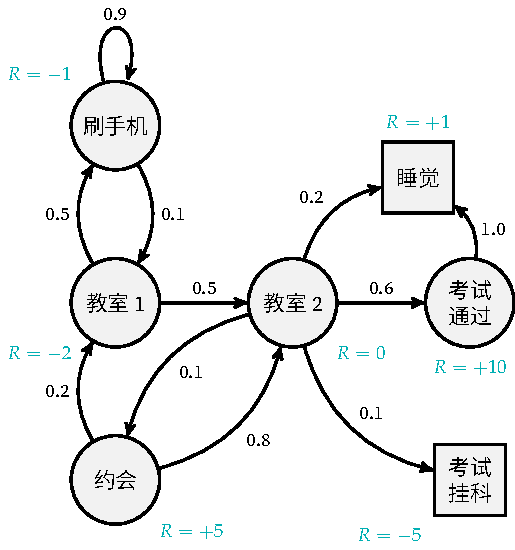
\includegraphics[width=0.7\textwidth]{figures/Markov-chain/STR.pdf}
    \caption{学生MRP}
    \label{fig:student-MRP}
\end{figure}

李二除了会获得即时奖励,他还会对未来有预期. 例如,尽管李二不愿意学习,但是考试通过的奖励是$+10$,为了这么大的奖励,现在遭罪一些是值得的,所以他会愿意坐在教室1里自习. 假如下一刻李二就要考试,这一刻他开始在教室1中自习,他对于下一刻考试通过的奖励预期是$+9$. 也就是说,李二对未来的奖励会有一个折扣,这个折扣因子就是$\gamma=9/10=0.9$.
\end{example}

更一般地,我们可以形式上定义MRP.

\begin{definition}[Markov奖励过程,MRP]
一个\textbf{Markov奖励过程}(\textbf{Markov奖励模型},\textbf{MRP})由四元组$\langle\calS,\calP,\mathcal R,\gamma\rangle$构成:
\begin{itemize}
    \item $\calS$是一个有穷的状态集合.
    \item $\calP$是一个状态转移矩阵,从$i$转移到$j$的概率记为$\calP_{i,j}$. 根据这一转移矩阵可以产生一个状态转移的Markov链$\{S_t\}_{t\geq 0}$.
    \item $\mathcal R$是(单步期望)奖励函数,定义为$\mathcal R_s = \E[\contrastlight{R_{t+1}}|S_t=s]$,其中,随机变量$\contrastlight{R_{t+1}}$表示下一阶段所处状态的奖励. 也就是说,当$t$时刻位于状态$s$时,$\mathcal R_s$是下一时刻获得的奖励的期望.
    \item $\gamma$是一个折扣因子,$\gamma\in[0,1]$.
\end{itemize}
\end{definition}

在MRP中,我们最关心的并不是实时奖励,而是综合来看整个过程的奖励. 为了描述这一点,我们引入\emph{回报}的概念.

\begin{definition}[回报]
MRP中,$t$时刻以后的总\textbf{回报}$G_t$定义为
    \[G_t = R_{t+1}+\gamma R_{t+2} +\dots =\sum_{k=0}^\infty \gamma^kR_{t+k+1}.\]    
\end{definition}
从定义中可以看到,$\gamma \in[0,1]$衡量了未来下一时段单位奖励在当前时刻的价值,$\gamma$越小,我们更偏好即时奖励,因而更“短视”;$\gamma$越大,我们更偏好未来奖励,因而更有“远见”.

我们这里对折扣做了极大的简化. 折扣因子和时间、状态都有可能有依赖关系. 
\begin{itemize}
    \item 在李二的例子中,他可能更愿意十天后有一次约会,而不是通过考试,换言之,约会对他的折扣因子可能是$0.99$,而考试通过的折扣因子可能是$0.9$.
    \item 如果老师给李二布置的作业难度波动很大,那么李二做完作业之后对通过考试的折扣因子就会发生变化:作业简单,李二觉得自己已经掌握了知识,对通过考试的折扣因子就会降低;作业困难,李二觉得自己可能很难通过考试,对通过考试的折扣因子就会提高.
\end{itemize}
然而,在MRP的定义中,我们假设了一个固定的折扣因子,并且规定了一个简单的方法计算折扣:$t$时刻后的奖励是即时奖励的$\gamma^t$倍. 这一定义体现了折衷的思想:如果折扣因子太符合实际,那么这个模型就不太实用. 在我们的定义之下,随着时间改变,折扣因子会指数衰减,这不仅和实验结果比较符合,而且也使得Markov性能被很好利用.

除了回报之外,在MRP中,我们更关心的是\emph{价值函数},即处于某个状态时候预期的回报是多少:
\begin{definition}[价值函数]
在MRP中,\textbf{状态-价值函数}(或\textbf{价值函数})定义为
    \[v(s) = \E[G_t|S_t=s].\]
\end{definition}

注意,等式右边有$t$但左边没有,所以我们需要说明这个定义对任意$t$都是成立的. 我们只需要说明对于任意的$t$,$t+1$和$t$定义了同一个$v(s)$. 注意,随机变量$R_{t+k}$只依赖于$S_{t+k}$,即$R_{t+k}=R(S_{t+k})$,所以
\begin{align*}
    \E[G_t|S_t=s] &= \E\left[\sum_{k=0}^\infty \gamma^k R_{t+k+1}\middle|S_t=s\right] \\
    &= \E\left[\sum_{k=0}^\infty \gamma^k R(S_{t+k+1})\middle|S_t=s\right]\\
    &= \sum_{k=0}^\infty \gamma^k \E[R(S_{t+k+1})|S_t=s].
\end{align*}
注意,项$\E[R(S_{t+k+1})|S_t=s]$的定义满足Markov性,即
\[\E[R(S_{t+k+1})|S_t=s]=\E[R(S_{t+k+2})|S_{t+1}=s].\]
因而对于任意的$t$,$t+1$和$t$定义了同一个$v(s)$.

因此,这一定义蕴含了Markov性:只从当前起考虑未来收益,不考虑历史收益(沉没成本)的影响;也蕴含了时齐性:价值函数的定义不依赖于时刻$t$(无穷阶段情形). 我们在后面要各种相关概念的定义都需要用到这个性质,证明都是类似的,不再赘述.

接下来我们展示价值函数的计算方法. 直观上说,回报应该被被分解为两部分:\contrastlight{即时回报$R_{t+1}$}以及\light{未来的回报$\gamma v(S_{t+1})$},也就是下一个状态期望回报再做折扣. 具体来说,我们有
\begin{align*}
v(s) &= \E(G_t|S_t=s) \\
    &= \E(R_{t+1}+ \gamma R_{t+2} + \gamma^2 R_{t+3}+\dots | S_t= s) \\
    &= \E(R_{t+1} + \gamma (R_{t+2}+\gamma R_{t+3}+\dots) | S_t = s) \\
    &= \E(R_{t+1} + \gamma G_{t+1} | S_t = s) \\
    &= \E(R_{t+1} | S_t = s) + \gamma \E(G_{t+1} | S_t = s) \\
    &= \E(\contrastlight{R_{t+1}}|S_t=s) + \E[\light{\gamma v(S_{t+1})}|S_t=s]\\
    &= \contrastlight{\mathcal R_s} + \light{\gamma \sum_{s'\in \calS}\calP_{s,s'}v(s')}.
\end{align*}
其中倒数第二行是因为
\begin{align*}
    \E(G_{t+1}|S_t=s) &= \sum_{s'\in \calS}\E(G_{t+1}|S_{t+1}=s',S_t=s)\Pr(S_{t+1}=s'|S_t=s)\\
    &= \sum_{s'\in \calS}\E(G_{t+1}|S_{t+1}=s')\Pr(S_{t+1}=s'|S_t=s)\\
    &= \sum_{s'\in \calS}v(s')\Pr(S_{t+1}=s'|S_t=s)\\
    &=\E[v(S_{t+1})|S_t=s].
\end{align*}
我们因此得到了\textbf{Bellman方程}:
\begin{theorem}[Bellman方程]\label{thm:MRP-Bellman}
    $v(s)=\mathcal R_s + \gamma \sum_{s'\in \calS}\calP_{s,s'}v(s')$.
\end{theorem}

在后面,我们将不断看到这样形式的方程,它将一个和Markov链有关的计算分解为当前的部分和未来的部分. 我们将这样形式的方程统称Bellman方程. 

Bellman方程可以用矩阵形式表达:
        \[v = \mathcal R + \gamma \mathcal P v.\]
这里$v$是列向量$v=(v(s))_{s\in\calS}$.

写成矩阵形式之后,我们可以看到,Bellman方程其实是一个线性方程,可以被直接解\footnote{这里我们假设$\gamma\neq 1$,否则这个方程是奇异的.}:
\[
    v =\mathcal R + \gamma \calP v \implies (I-\gamma \calP)v = \mathcal R \implies v = (I-\gamma \calP)^{-1} \mathcal R.
\]
我们还可以有另一种观点,考虑一个映射$f:\calS\to \calS$,$f(v)=\mathcal R + \gamma \calP v$,那么Bellman方程可以被写作
\[v=f(v).\]
因此,$v$是$f$的\emph{不动点}. 在\Cref{chap:fixed-point-theory},我们将系统地讨论不动点的性质以及它对于Markov链相关模型的重要性.

回到解Bellman方程,对于$n$个状态的Markov链,用线性方程组法的计算复杂度为$\O(n^3)$. 对于较小的MRP可以直接解,太大的MRP开销太大. 对于大型MRP,可以采用迭代算法,例如:
\begin{itemize}
    \item 动态规划
    \item Monte-Carlo评估
    \item 时序差分学习
\end{itemize}
动态规划法的思路我们将在\Cref{sec:HMM}中介绍.

\section{Markov决策过程(MDP)}\label{sec:MDP}

上一节中我们建模了Markov链上的价值系统,即MRP,接下来我们进入建模决策的环节. 回顾李二的例子(\Cref{ex:lier-MRP}),我们在MRP中忽略了一个非常重要的考虑:当李二坐在教室1中的时候,李二不是随机地开始刷手机的,他需要\emph{选择}开始刷手机. 换言之,在MRP中,在当前状态可以做什么\emph{行动}是缺失的. 

此外,李二的奖励其实不是由状态决定的,而是由他做了什么行动决定的,这样,李二才能评估做什么行动可以最大化自己的奖励,然后选择奖励高的那个行动. 实际上,认知神经科学的研究表明,人体的运动控制就是由类似的机制完成的:首先,大脑皮层会提出若干不同的运动计划,这些运动计划对应了不同的奖励(由多巴胺浓度来表征),人脑中有一个被称作基底神经节的结构,它负责“放行”奖励高于某个阈值的运动计划,于是人就可以产生这个动作了. 

综合以上这些思考,我们就可以给出\emph{Markov决策过程}(MDP)的模型. 我们还是先看李二的例子,然后再推广到一般的情况. 

\begin{example}[李二MDP]
李二的MDP见\Cref{fig:studentMDP}. 
\begin{figure}
    \centering
    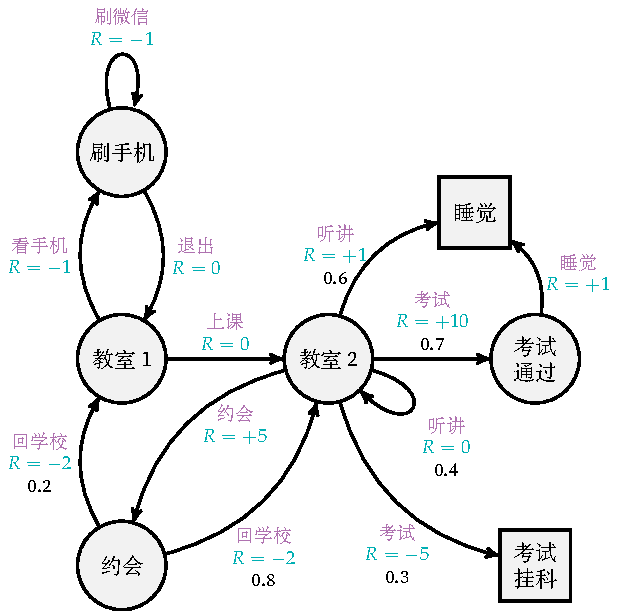
\includegraphics[width=0.75\textwidth]{figures/Markov-chain/STD.pdf}   
    \caption{学生MDP}
    \label{fig:studentMDP}
\end{figure}
在图中,状态依然是之前状态,但是状态的转移被给上了两个标签:
\begin{enumerate*}[label=(\arabic*)]
    \item 这个转移是什么动作引起的(紫色),
    \item 这个动作可以带来多少的奖励(蓝色). 
\end{enumerate*}
例如,当李二在教室1的时候,她如果选择看手机,那么就会有$-1$的奖励,并且进入刷手机的状态. 
\end{example}

接下来,我们给出一般的MDP的定义.
\begin{definition}[Markov决策过程,MDP]
\textbf{Markov决策过程}(\textbf{MDP})是一个MDP是五元组$\langle\calS, \light{\mathcal A}, \calP, \mathcal R, \gamma\rangle$,其中
\begin{itemize}
    \item $\calS$是一个有限的状态集合.
    \item $\light{\mathcal A}$是一个有限的\emph{行动}(action)集合.
    \item $\calP$是状态转移概率矩阵,
    \[\calP_{ss'}^{\light{a}} = \Pr(S_{t+1} = s' | S_t = s, A_t = \light{a}).\]
    \item $\mathcal R$是一个奖励函数,$\mathcal R_s^{\light{a}} = \E(\contrastlight{R_{t+1}} | S_t = s, A_t = \light{a})$,随机变量$\contrastlight{R_{t+1}}$是进行某一行动到达某一状态后的奖励.
    \item $\gamma$是一个折扣因子$\gamma\in[0,1]$.
\end{itemize}
\end{definition}

现在我们对比MDP和MRP. MDP中,状态转移矩阵依赖动作,奖励函数也依赖动作. 在李二的例子中,在教室2如果选择听讲,尽管都是在听讲,但是并不一定会产生一个确定的结果:他会有$0.4$的概率睡着,$0.6$的概率继续听讲. 自然,睡着的奖励和继续听讲的奖励是不同的.

\begin{definition}[策略]
一个\emph{策略}$\pi$是给定状态下行动的分布,即对任意$s\in\calS$和$a\in\mathcal A$,有
    \[\pi(a|s) = \Pr(A_t=a | S_t = s).\]
\end{definition}
一个策略完全决定了一个智能体在MDP环境中的行为. 它的定义蕴含着Markov性:MDP的策略取决于当前状态,而非历史状态;也蕴含着时齐性:MDP的策略不依赖于时刻$t$. 这样的定义会方便我们讨论价值函数以及决策的问题.

MDP与MDP的关系由策略给出. 
\begin{proposition}
给定一个MDP $\calM=\langle\calS,\mathcal A,\calP,\mathcal R, \gamma\rangle$和一个策略$\pi$,$\langle \calS, \calP^{\pi}\rangle$是一个Markov链,$\langle\calS,\calP^{\pi}, \mathcal R^{\pi}, \gamma\rangle$是一个MRP,其中
\[\calP_{s,s'}^{\pi} = \E_{a\sim\pi(\cdot|s)}(\calP^a_{s,s'})=\sum_{a\in \mathcal A}\pi(a|s)\mathcal P_{s,s'}^{a},\]
    \[\mathcal R_s^{\pi} =\E_{a\sim\pi(\cdot|s)}(\mathcal R^a_s)=\sum_{a\in\mathcal A}\pi(a|s)\mathcal R_s^a.\]
\end{proposition}
\begin{proof}
对行动利用全概率公式. 
\end{proof}

现在我们有三个概念,MDP, MRP,以及Markov链,\Cref{prop:state-action-value} 给了他们三者的关系,我们可以总结到\Cref{fig:MDP-MRP-MarkovChain}. 

\begin{figure}[ht]
\centering

\includegraphics[width=0.8\textwidth]{figures/Markov-chain/MDP-MRP-Markov-chain.pdf}
\caption{MDP,MRP和Markov链的关系}\label{fig:MDP-MRP-MarkovChain}
\end{figure}

对于李二来说,选择什么样的策略很大程度取决于他能从中获得多少奖励. 同样,在MDP中,我们可以定义\emph{回报}的概念. 

\begin{definition}[回报]
在MDP中,$t$时刻以后的总\textbf{回报}$G_t$定义为
    \[G_t = R_{t+1} + \gamma R_{t+2} + \gamma^2 R_{t+3} + \dots = \sum_{k=0}^\infty \gamma^k R_{t+k+1}.\]
\end{definition}

类似MRP,我们需要定义相应的\emph{价值函数}. 在MDP中,\emph{状态-价值函数}和\emph{行动-价值函数}是两个重要的价值函数,它们分别描述了从某一状态出发,遵从某一策略的期望回报. 

\begin{definition}[价值函数]
\textbf{状态-价值函数} $v_\pi(s)$ 是从状态$s$出发,遵从策略$\pi$的期望回报
    \[v_\pi(s) = \E_\pi(G_t|S_t=s).\]

\textbf{行动-价值函数} $q_\pi(s,a)$ 是从状态$s$出发,采取行动$a$,遵从策略$\pi$的期望回报
    \[q_\pi(s,a) = \E_\pi(G_t|S_t=s,A_t=a).\]
\end{definition}
注意,类似MRP中的价值函数,MDP中的价值函数定义也不依赖$t$的选择,这是因为MDP的Markov性和时齐性. 

行动-价值函数比起状态-价值函数更加具体,它可以帮助李二评判在当前选择每一个行动的回报,从而选择最优的行动. 而状态-价值函数则是对行动-价值函数的一个期望,因而是李二预期他从这个状态出发的回报. 具体来说,这两个价值函数有如下关系:

\begin{proposition}\label{prop:state-action-value}
状态-价值函数$v_\pi(s)$和行动-价值函数$q_\pi(s,a)$之间有如下关系:
    \[v_\pi(s) = \E_{a\sim\pi(\cdot|s)}(q_\pi(s,a))=\sum_{a\in\mathcal A}\pi(a|s)q_\pi(s,a),\]
    \[q_\pi(s,a) =\mathcal R_s^a + \gamma \sum_{s'\in \calS}P_{s,s'}^a v_\pi(s').\]
\end{proposition}
\begin{proof}
    用$q_\pi(s,a)$来表示$v_\pi(s)$,对行动$a$用全概率公式即可得到. 

    另一方面,用$v_\pi(s)$来表示$q_\pi(s,a)$也是全概率公式. 具体来说,在状态$s$采取行动$a$之后,期望上有$\mathcal R_s^a$的即时奖励,然后以$\calP_{s,s'}^a$的概率转移到状态$s'$,在状态$s'$的期望回报是$\gamma v_\pi(s')$. 按照$s'$用全概率公式即可得到$q_\pi(s,a)$.
\end{proof}

下面我们给出状态-价值函数和行动-价值函数的Bellman方程. 首先,价值函数可以被分解为\contrastlight{\emph{即时回报}}加\light{\emph{未来的折扣回报}},具体来说
\begin{itemize}
    \item 状态-价值函数可以被分解为:
    \[v_\pi(s) = \E_\pi[\contrastlight{R_{t+1}} + \light{\gamma v_\pi(S_{t+1})}|S_t=s].\]
    \item 行动-价值函数可以被类似地分解,
\[q_\pi(s,a) = \E_\pi[\contrastlight{R_{t+1}} + \light{\gamma q_\pi(S_{t+1},A_{t+1})}|S_t=s,A_t=a].\]
\end{itemize}

他们的计算方法和\Cref{thm:MRP-Bellman} 中的方法类似. 继续仿照\Cref{thm:MRP-Bellman} 的证明,我们可以得到MDP的Bellman方程:

\begin{theorem}[Bellman方程]
\[v_\pi(s) = \sum_{a\in \mathcal A}\pi(a|s)\left(\mathcal R_s^a + \gamma \sum_{s'\in \calS}\calP_{s,s'}^av_\pi(s')\right),\]
\[q_\pi(s,a) = \mathcal R_s^a + \gamma \sum_{s'\in \calS}\calP_{s,s'}^a \sum_{a'\in \mathcal A}\pi(a'|s')q_\pi(s',a').\]
\end{theorem}

状态-价值函数的Bellman方程可以被写成矩阵形式:
\[v_\pi = \mathcal R^\pi + \gamma \calP^\pi v_\pi = (I-\gamma \mathcal P^\pi)^{-1}\mathcal R^\pi.\]

注意,MDP的Bellman方程只能告诉我们给定策略$\pi$的价值函数,它并不能告诉智能体(也就是李二)要如何行动,所以,接下来我们要讨论最优策略和最优价值函数. 

\begin{definition}[最优价值函数]
\textbf{最优状态-价值函数} $v_\star(s)$ 是所有策略中最大的状态-价值函数
    \[v_\star(s) = \max_\pi v_\pi(s).\]

\textbf{最优行动-价值函数} $q_\star(s,a)$是所有策略中最大的行动-价值函数
    \[q_\star(s,a) = \max_\pi q_\pi(s,a).\]
\end{definition}

相应地,最优价值函数确定了智能体在MDP中的最佳收益,解MDP即确定达到最优价值函数的策略. 

在以上定义中可能会遇到这样的问题:对两个状态$s_1$和$s_2$,存在两个不同的策略$\pi_1$和$\pi_2$,使得$v_\star(s_1)=v_{\pi_1}(s_1)$,$v_\star(s_2)=v_{\pi_2}(s_2)$. 此时,每个状态取到最大价值的策略$\pi$可能并不是同一个,因此$v_\star$并不是某个特定策略可以实现的值. 所以,我们需要证明,存在一个策略$\pi_\star$,使得对于任意的策略$\pi$,$\pi_\star$都取得最大价值函数. 

我们有如下定理,说明了这样策略的存在性,因而也证明了MDP解的存在性. 
\begin{theorem}[MDP解的存在性]\label{thm:MDP-existence}
对任意MDP,存在一个策略$\pi_\star$,
\begin{itemize}
    \item 对任意状态$s$,$v_{\pi_\star}(s) = v_\star(s)$.
    \item 对任意状态$s$和行动$a$,$q_{\pi_\star}(s,a)=q_\star(s,a)$.
\end{itemize}
\end{theorem}

\begin{proof}
我们给出一个构造性证明,即找出最优策略. 我们先找到一个$\pi_\star$最大化$q$,然后说明这个$\pi_\star$也可以最大化$v$. 

直观上说,我们只要对每个状态都选择最好的行动,这就是一个最优策略. 具体来说,我们可以通过如下步骤找到$\pi_\star$:
\begin{itemize}
    \item 固定$s$,
    \item 找到一个$a_\star$最大化$q_\star(s,\cdot)$,即$q_\star(s,a_\star)=\max_{a}q_\star(s,a)$,令$\pi_\star(a_\star|s)=1$.
    \item 对其他$a\neq a_\star$,令$\pi_\star(a|s)=0$.
\end{itemize}
首先,根据选法,$\pi_\star$取得最优行动-价值函数. 接下来我们说明,它也取得了最优状态-价值函数. 任意策略$\pi$,给定状态$s$,我们有如下计算:
\begin{align*}
    v_\pi(s) &= \E_{a\sim\pi(\cdot|s)}[q_\pi(s,a)]\\
             &\leq \E_{a\sim\pi(\cdot|s)}[q_\star(s,a)]\\
             &\leq q_\star(s,a_\star)\\
             &=v_{\pi_\star}(s).
\end{align*}
\end{proof}
这个证明还有一个推论:
\begin{corollary}
    对任意MDP,总存在一个非随机的最优策略,即对任意状态$s$,$\pi_\star(a|s)\in\{0,1\}$.
\end{corollary}

两个最优价值函数之间有如下关系:
\begin{proposition}\label{prop:state-action-value-optimal}
\[v_\star(s) = \max_a q_\star(s,a),\]
\[q_\star(s,a) = \mathcal R_s^a + \gamma \sum_{s'\in \calS}\calP_{s,s'}^av_\star(s').\]
\end{proposition}
\begin{proof}
    在\Cref{thm:MDP-existence} 的证明中,我们将$\pi$取为$\pi_\star$,于是有
    \[v_\star(s) = v_{\pi_\star}(s) = q_{\star}(s,a_\star) = \max_a q_\star(s,a).\]
    对于第二个等式,根据\Cref{thm:MDP-existence},
    \[v_\star(s) = v_{\pi_\star}(s),\quad q_\star(s,a) = q_{\pi_\star}(s,a),\]
    在\Cref{prop:state-action-value} 取$\pi=\pi_\star$即可得到.
\end{proof}

根据上面结论,如果我们知道$q_\star(s,a)$或者$v_\star(s)$,我们就能获得最优策略. 这一计算同样依赖Bellman方程\footnote{在文献中,这一Bellman方程被称为Bellman\emph{最优性}方程,而之前推导的Bellman方程被称为Bellman\emph{期望}方程. 为了不过度引入术语,我们这里不做这种区分. }:

\begin{theorem}[Bellman方程]
\[v_\star(s) = \max_a\left\{\mathcal R_s^a + \gamma \sum_{s'\in \calS}\calP_{s,s'}^av_\star(s')\right\},\]
\[q_\star(s,a) = \mathcal R_s^a+\gamma \sum_{s'\in \calS}\calP_{s,s'}^a\max_{a'}q_\star(s',a').\]
\end{theorem}
\begin{proof}
    对于第一个方程,将\Cref{prop:state-action-value-optimal} 中第二个等式代入第一个等式即可得到. 

    对于第二个方程,将\Cref{prop:state-action-value-optimal} 中第一个等式代入第二个等式即可得到. 
\end{proof}

Bellman不是线性的. 因此很难有解析形式的解. 但是MDP的数值解是可以多项式时间求出来的. 我们一般采用迭代算法求解:
\begin{itemize}
    \item 价值迭代
    \item 策略迭代
    \item Q-learning
    \item Sarsa
\end{itemize}

求解MDP的过程实际上就是人工智能中\emph{强化学习}的核心步骤. 在本节的开头,我们说过人脑运动控制机制. 实际上,绝大部分的哺乳动物都具备类似这样的学习机制:通过奖励的反馈,动物可以学会如何行动,从而获得最大的奖励. 这样的学习机制被称为\emph{强化学习}. 强化学习在很多复杂交互的环境中都有广泛的应用,例如围棋的AlphaGo、星际争霸的AlphaStar 等.

\begin{remark}
Bellman方程是\emph{强化学习}、经济学\emph{动态优化}的核心. Bellman方程的推导是Markov链中最为常用的技巧:考虑从当前状态转移到下一状态,利用全概率公式,一步转移会将两个状态之间的概率(期望)用递推公式联系起来. 在随机过程中,有大量这样的例子:\emph{前向方程}、\emph{Wald等式}、\emph{调和函数}. 后面的\emph{HMM}也是类似的例子.    
\end{remark}

最后,我们谈谈深度强化学习. 在一些非常复杂的情况下(例如下围棋),使用经典的迭代算法并不容易求解MDP. \emph{深度强化学习}是一种结合了深度学习和强化学习的方法. 在深度强化学习中,用神经网络来表示$\pi$和$v$,之后,用某种学习算法训练神经网络. 

在一些深度强化学习模型中(例如AlphaZero),状态空间$\calS$也用一个神经网络表示. 用神经网络来表示状态空间的好处是可以减少人类的特征工程,让神经网络充分发掘状态空间好的表示方法.

在很多深度强化学习模型中(例如AlphaGo),MDP的策略是基于过去$k$期的状态做当前的决策,这样可以更好地利用状态的历史信息. 这样的决策模型等价于一个利用一期信息决策的MDP(见习题\lhysays{出一下}),因此依然可以用同样的深度学习算法来求解. 


\section{隐Markov模型(HMM)}\label{sec:HMM}

在本节,我们考虑Markov链上的另一种应用. 在统计学和机器学习中,我们有时候要处理一类含时间的数据. 例如,如果我们希望利用机器的力量帮助我们炒股赚钱,就要考虑如何预测股价然后做出相应的决策,这样的投资模式被称为\emph{量化投资}. 在1989年到2009年间,量化界的传奇人物James Simons操盘大奖章基金,平均年回报率高达35\%,即便是在次贷危机爆发的2007年,该基金的回报率仍高达85\%. 据说,让Simons成功的秘诀是\emph{隐Markov模型},这正是本节的主题.

我们先给出隐Markov模型的定义. 

\begin{definition}[隐Markov模型,HMM]
一个\textbf{隐Markov模型}(\textbf{HMM}) 是两列随机变量(被称为\emph{观测序列})$X_1,X_2,\dots,$和$z_1,z_2,\dots,$(被称为\emph{隐状态序列})的序列,满足:
    \begin{itemize}
        \item $\{Z_t\}$构成一条Markov链.
        \item 对任意$t$,$X_t$的分布仅依赖于$Z_t$.
        \item 对于任意$t$,$\Pr(X_t|Z_t)$服从分布$F(Z_t)$.
    \end{itemize}
\end{definition}
示意见\Cref{fig:HMM}.
\begin{figure}[ht]
    \centering
    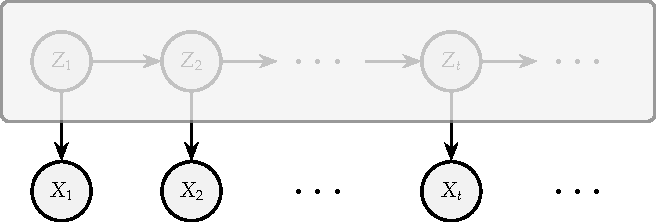
\includegraphics[width=0.8\textwidth]{figures/Markov-chain/HMM.pdf}
    \caption{隐Markov模型}
    \label{fig:HMM}
\end{figure}    

为了理解这一概念,我们可以考虑炒股的例子. 
\begin{example}[美为HMM]\label{ex:meiwei-HMM}
假设我们要投资美为的股票,第$t$天的股票价格是$X_t$. 我们很希望理解整个$X_t$的变化趋势. 然而,美为股价的背后有一个神秘势力操控. 我们并不清楚这个神秘势力每天决策的具体细节,只知道他们的决策非常健忘,即他们的决策只依赖于前一天的决策. 他们会决定一个明天的预计股价$Z_t$,这构成了一个Markov链$\{Z_t\}$. 

因为市场和汇率的波动,这个神秘势力无法完全决定股票的价格$X_t$,然而,他们每一天所决定的预期价格$Z_t$会导致股票价格的变化,我们可以认为$X_t$仅依赖于$Z_t$,但依然受到一些随机因素的影响. 作为简化,我们假设每天的随机影响是独立且一致的,服从分布$F(Z_t)$. 这样的得到的模型就是一个HMM.
\end{example}

接下来,我们给HMM引入一些记号. 为简便起见,我们只研究有限离散的HMM. 设HMM $\calM$所形成的概率测度是$\Pr_\calM$. 我们假设模型中以下的量都是已知的:
\begin{itemize}
    \item $\mathcal Z$: 有限的状态集合,即$Z_t$的取值集合.
    \item $\mathcal X$: 有限的观测集合,即$X_t$的取值集合.
    \item $T$:Markov链$\{Z_t\}$的转移矩阵,$T_{i,j}=\Pr_\calM(Z_{t+1}=j|Z_t=i)$.
    \item $M$:给定隐状态时的观测概率,$M_{i,k} = \Pr(X_t=k|Z_t=i)$.
    \item $\lambda$:隐状态的初始分布.
\end{itemize}

我们会把序列$A_i,\dots, A_j$记作$A_{i:j}$,然后将它看作一个向量. 例如$X=X_{1:t}$就是描述从时刻$1$到$t$的观测序列的随机向量,而$Z=Z_{1:t}$就是描述从时刻$1$到$t$的隐状态序列的随机向量.

为了理解HMM的任务,我们接着看美为的例子. 假设我们已经知道一个HMM $\calM$可以预测美为的股价$X_t$,作为一个使用者,我们希望$\calM$确实有用. 因此,我们要\emph{评估}这个模型的表现. 具体来说,我们希望知道,给定观测历史$x=(x_1,x_2,\dots,x_t)$,如何计算$\Pr_\calM(X=x)$. 这一方法也可以用来做\emph{预测}:利用全概率公式,我们可以计算$\Pr_\calM(X_{t+1}=x_{t+1}|X=x)$,从而预测未来的股价.

评估一个HMM固然重要,但是评估依然是把HMM当成一个黑盒来使用. 我们还希望知道这个模型背后到底发生了什么,这就是\emph{解释}问题. 具体来说,我们希望知道,给定观测历史$x=(x_1,x_2,\dots,x_t)$以及一个时刻$k$,如何计算$\Pr_\calM(Z_k|X=x)$. 这一分布表明了在$k$时刻神秘势力更有可能做了什么样的决策,从而帮助我们更好理解股价的波动.

接下来我们将分别阐述如何解决评估问题和解释问题. 因为我们只讨论某一个具体的HMM,为简便起见,我们此后都将概率测度$\Pr_\calM$简记为$\Pr$.

\subsection{评估问题}

我们引入记号随机向量$X=(X_1,\dots,X_t)$,$Z=(Z_1,\dots,Z_t)$. 我们考虑HMM的\emph{评估}问题:给定一个HMM $\calM$,以及它的观测历史$x=(x_1,x_2,\dots,x_t)$,计算$\Pr(X=x)$. 

关键困难是我们不知道隐状态历史$Z=(z_1,z_2,\dots,z_t)$,因此我们需要利用全概率公式将隐状态消除掉,即:
\[
    \Pr(X=x) =\sum_{Z=(z_1, \dots, z_t) \in \mathcal Z^t} \light{\Pr(X=x|Z=z)}\contrastlight{\Pr(Z=z)}.
\]
接下来我们分别计算$\light{\Pr(X=x|Z=z)}$和$\contrastlight{\Pr(Z=z)}$. 对于前者,因为每一个观测值$X_i$仅依赖于$Z_i$,我们有
\[
    \light{\Pr(X=x|Z=z)} = \prod_{i=1}^t \Pr(X_i = x_i| Z_i = z_i) = M_{z_1,x_1}\cdot M_{z_2,x_2}\dots M_{z_t,x_t},
\]
对于后者,因为$Z$是一个Markov链,我们有
\begin{align*}
    \contrastlight{\Pr(Z=z)} &= \Pr(Z_1 = z_1) \prod_{i=2}^t\Pr(Z_i = z_i| Z_{i-1} = z_{i-1}) 
    \\
    &= \lambda_{z_1}\cdot T_{z_1,z_2}\cdot T_{z_2,z_3}\dots T_{z_{t-1},z_t}.
\end{align*}

以上的量都是已知的,所以我们已经可以计算评估问题了. 然而,这一方法的需要计算的乘法次数是$\O(t|\mathcal Z|^t)$,对于很大的$t$和$\mathcal Z$,这是不可接受的计算量. 我们需要更好的计算方法.

接下来,我们采用前向方程(见\Cref{thm:kolmogorov-chapman})的思路,从前$k$步的结果推出前$k+1$步的结果,然后据此列出递推方程. 在第$k+1$步,Markov链的状态发生了转移,按照从哪个状态转移到了哪个状态,我们可以拆分概率:
\begin{align*}
      &\Pr(X_{1:k+1}=x_{1:k+1}) \\
    = &\sum_{z\in \mathcal Z}\Pr(X_{1:k}=x_{1:k}, Z_k=z)\Pr(X_{k+1}=x_{k+1}|Z_k=z)\\
    = &\sum_{z\in \mathcal Z}\Pr(X_{1:k}=x_{1:k}, Z_k=z)\sum_{z'\in \mathcal Z}\Pr(Z_{k+1}=z'|Z_k=z)\Pr(X_{k+1}=x_{k+1}|Z_{k+1}=z')\\
    = &\sum_{z\in \mathcal Z}\Pr(X_{1:k}=x_{1:k}, Z_k=z)\sum_{z'\in \mathcal Z}T_{z,z'}M_{z',x_{k+1}}.
\end{align*}
如果把左边按照$Z_{k+1}$拆分,我们有
\[
    \sum_{z\in\mathcal Z}\light{\Pr(X_{1:k+1}=x_{1:k+1}, Z_{k+1}=z)} = \sum_{z\in \mathcal Z}\light{\Pr(X_{1:k}=x_{1:k}, Z_k=z)}\sum_{z'\in \mathcal Z}T_{z,z'}M_{z',x_{k+1}}.
\]
如果令$\light{\alpha_k(z):=\Pr(X_{1:k}=x_{1:k}, Z_k=z)}$,用类似的计算,我们有递推:
\begin{itemize}
    \item 当$k=1$,$\light{\alpha_k(z)} = \lambda(z)M_{z,x_k}$.
    \item 当$k>1$,$\light{\alpha_{k+1}(z)} = \sum_{z' \in \mathcal Z}\light{\alpha_{k}(z')}T_{z',z}M_{z,x_{k+1}}$.
\end{itemize}
最后,$\Pr(X=x) = \sum_{z\in \mathcal Z}\light{\alpha_t(z)}$. 这一方法需要算的乘法次数是$\mathcal O(t|\mathcal Z|^2)$,比前一种计算方法要快很多.

镜像地,我们可以使用后向方程的思路,从前$k+1$步的结果推出前$k$步的结果. 同样可以列出递推方程. 定义$\beta_k(z):=\Pr(X_{k+1:t}=x_{k+1:t} | Z_k=z)$,我们有递推:
\begin{itemize}
    \item 当$k = t$,$\beta_k(z) = 1$.
    \item 当$1 \leq k < t$,$\beta_{k}(z) = \sum_{z' \in \mathcal Z}T_{z,z'}M_{z',x_{k+1}}\beta_{k+1}(z')$.
\end{itemize}
于是,$\Pr(X=x) = \sum_{z\in \mathcal Z}\lambda(z)M_{z,x_1}\beta_1(z)$. 这一方法需要算的乘法次数是$\mathcal O(t|\mathcal Z|^2)$.


\subsection{解释问题}
接下来我们讨论HMM的\emph{解释问题}. 给定一个 HMM $\calM = (\mathcal Z, \mathcal X, T, M, \lambda)$, 一列观测历史$x = (x_1, x_2, \dots, x_t)$, 解释问题旨在寻找一个状态序列,能最好地解释这些历史观察. 具体来说我们考虑如下四个问题:
\begin{enumerate}
    \item \emph{过滤}:计算$\Pr(Z_k = s|X_{1:k}=x_{1:k})$.
    \item \emph{平滑}:计算$\Pr(Z_k = s|X=x)$,$k < t$.
    \item \emph{预测}:计算$\Pr(Z_k = s|X=x)$,$k > t$.
    \item \emph{解码}:找到最有可能的状态序列 $z = (z_1, z_2, \dots, z_t)$.
\end{enumerate}

首先考虑过滤:$\Pr(Z_k = s|X_{1:k}=x_{1:k})$. 回顾记号$\alpha_k(s)= \Pr(X_{1:k}=x_{1:k}, Z_k=s)$,这其实已经足够我们计算过滤了. 根据条件概率的定义,我们有
\begin{align*}
    \Pr(Z_k = s|X_{1:k}=x_{1:k}) & = \frac{\Pr(X_{1:k}=x_{1:k}, Z_k=s)}{\Pr(X_{1:k}=x_{1:k})} \\
    &= \frac{\alpha_k(s)}{\sum_{z\in\mathcal Z}\alpha_k(z)}.
\end{align*}
我们已经知道如何计算$\alpha_k(s)$,所以这就可以用来计算过滤了.

然后是平滑:$\Pr(Z_k = s|X=x)$,$k < t$.  回顾记号$\alpha_k(s)= \Pr(X_{1:k}=x_{1:k}, Z_k=s)$,以及$\beta_k(s)=\Pr(X_{k+1:t}=x_{k+1:t} |Z_k=s)$. 可以证明(见习题\lhysays{出一下}):
\begin{equation}
    \Pr(z_k = s|X=x)=\frac{\beta_k(s)\alpha_k(s)}{\sum_{z\in\mathcal Z}\alpha_t(z)}.\label{eq:smooth}
\end{equation}
同样,我们已经知道如何计算$\alpha_k(s)$和$\beta_k(s)$,所以这就可以用来计算平滑了.

之后是预测:$\Pr(Z_k = s|X=x)$,$k > t$. 首先用过滤计算 $\lambda=\Pr(Z_t = s|X=x)$. 从$t$之后的隐状态都只依赖于$t$时刻的隐状态$Z_t$,因此,条件在$X=x$下,$Z_t,Z_{t+1},\dots,Z_k$构成了一个Markov链,它的初始分布为$\lambda$,转移矩阵为$T$. 于是我们利用\Cref{thm:kolmogorov-chapman} 来计算该Markov链第$k-t$步的分布.

最后是解码:求$z=(z_1,z_2,\dots,z_t)$,使得$\Pr(Z=z|X=x)$最大. 注意,这一概率最大等价于$\Pr(Z=z,X=x)$最大. 我们也使用递归的想法来解决这个问题. 同样,在前$k-1$个状态已经选好之后,考虑最后一个状态应该选哪个. 具体来说,定义
    \[\delta_k(s) = \max_{z_{1:k-1}}\Pr(Z_{1:k} = (z_{1:k-1}, s), X_{1:k}=x_{1:k}).\]
于是
\begin{align*}
    &\delta_{k+1}(s) \\
    =& \max_{z_{1:k}}\Pr(Z_{1:k+1} = (z_{1:k}, s), X_{1:k+1}=x_{1:k+1})\\
    =& \max_{z_{1:k}}\{\Pr(Z_{1:k} = z_{1:k}, X_{1:k}=x_{1:k})\Pr(Z_{k+1}=s|Z_k=z_k) \Pr(X_{k+1}=x_{k+1}|Z_{k+1}=s)\}\\
    =& \max_{q}\{\max_{z_{1:k-1}}\Pr(Z_{1:k} = (z_{1:k-1},q), X_{1:k}=x_{1:k})T_{q,s}\}M_{s,x_{k+1}}\\
    =& \max_{q}\{\delta_k(q)T_{q,s}\}M_{s,x_{k+1}}.
\end{align*}
这就给出了从$k$推导到$k+1$的递推方程. 这一递推的初始状态是
\[\delta_1(s) = \Pr(Z_1=s, X_1=x_1) = \Pr(Z_1=s)\Pr(X_1=x_1|Z_1=s) = \lambda(s)M_{s,x_1}.\]

利用这一递推,我们就可以解决解码问题了. 具体算法在下面给出.
\begin{enumerate}
    \item 利用递推公式,逐层用第$k$层的$\delta_k$计算第$k+1$层的$\delta_{k+1}$,最后得到$\delta_t$. 
    \item 求一个$z_t^*$使得$\delta_t(z_t^*)$最大,根据定义,这个$z_t^*$也使得$\Pr(Z=z,X=x)$最大,把这个最大值记为$\delta^*_t$.
    \item 接下来,逐层用第$k+1$层的$\delta_{k+1}^*$计算第$k$层的$\delta_k^*$和$z_k^*$. 已知
    \[\delta_{k+1}^*=\delta_{k+1}(z_{k+1}^*)=\max_{q}\{\delta_k(q)T_{q,z_{k+1}^*}\}M_{z_{k+1}^*,x_{k+1}},\]
    从中找到一个$q$使得$\delta_k(q)T_{q,z_{k+1}^*}$最大,记此时的$\delta_k(q)$为$\delta_k^*$,$z_k^*=q$.
    \item 最后,我们就得到了最优的状态序列$z=(z_1^*,z_2^*,\dots,z_t^*)$,使得$\Pr(Z=z,X=x)$最大.
\end{enumerate}
以上算法被称为\emph{Viterbi算法},是解码问题的一个高效算法,它需要计算的乘法次数是$\O(t|\mathcal Z|^2)$. 这一算法采用了\emph{动态规划}的思想,实际上大部分和Bellman方程有关的问题(特别是最优化的问题)都可以用这一方法解决.

\section{扩散模型}

本节我们讨论基于Markov链的另一种模型,即扩散模型. 不同于之前的模型,扩散模型的启发来自物理学. 滴一滴墨水到水中,最后墨会均匀地在水中分布,这一过程不会反过来,即墨水不会自动聚集到一起. 同样的现象在热力学中也有体现:如果把金属勺子的一端放在热水中,热量会从热水中通过勺子传导到勺子的另一端,最终整个勺子会均匀地变热,而不会反过来. 这些现象都是\emph{扩散过程}. 本节的主要任务就是为这一过程建立数学模型,并讨论它的应用. 

我们先看墨水的例子. 
\begin{example}[墨水的扩散]\label{ex:ink-diffusion}
墨水的扩散有一个具体的数学模型,即\emph{Ehrenfest模型}. 

模型如\Cref{fig:ehrenfest-model} 所示. 在这个模型中,一共有两个箱子A和B,我们可以想象成这是水杯的上半部分和下半部分. 两个箱子里一共$N$个球,我们可以想象成这是墨水分子. 每个时刻,有很小的概率$\alpha>0$,盒子A和B中的球会保持不动;另外的$1-\alpha$的概率,我们均匀随机选择一个球,从一个箱子跳到另一个箱子,这就是扩散的过程. 

\begin{figure}[ht]
    \centering
    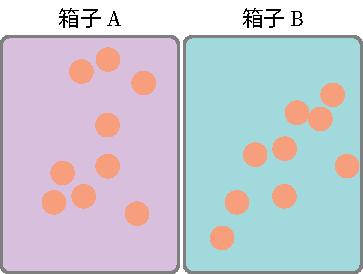
\includegraphics[width=0.5\textwidth]{figures/Markov-chain/Ehrenfest-model.pdf}
    \caption{Ehrenfest模型示意图}\label{fig:ehrenfest-model}
\end{figure}

设$X_k$是盒子A中球的数目,那么$\{X_k\}$是一个Markov链,它的转移核\footnote{我们在前面都说的是\emph{转移矩阵},然而,在扩散模型这一部分,\emph{转移核}是一个更恰当的表述. 这是因为,我们之前处理的大部分Markov链都是离散的状态空间,而这一部分处理的状态空间既有离散的也有连续的,所以“矩阵”并不是一个恰当的词汇. }是
\[
    \Pr(X_{k+1}=i|X_k=j) = \begin{cases}
        \alpha, & i = j,\\
        (1-\alpha)j/N, & i = j-1,\\
        (1-\alpha)(N-j)/N, & i = j+1,\\
        0, & \text{其他}.
    \end{cases}
\]

下面我们来解释为什么墨水最终会均匀分布在水中. 从遍历定理(\Cref{thm:ergodic-theorem})我们知道,对于一个遍历的Markov链,无论初始分布是什么,Markov链最终都会收敛到唯一平稳分布. 可以证明(见习题\lhysays{出一下}),$\{X_k\}$是一个遍历的Markov链,所以它会收敛到一个平稳分布$\pi\sim B(N,1/2)$. 

根据二项式的性质,该分布在$N/2$附近取到最大值,因此,这是墨分子最有可能的分布情况. 更精细的结论是(见习题\lhysays{出一下}),对任意$\epsilon>0$,当$N$充分大的时候,
\[
    \Pr\left(\limsup_{k\to\infty}\left|\frac{X_k}{N}-\frac{1}{2}\right|<\epsilon\right) \approx 1.
\]
换言之,几乎以概率$1$,分子会均匀分布在两个箱子中,即墨水会均匀地分布在水中.
\end{example}

以上例子告诉我们,物理过程几乎是不可逆的. 然而,如果我们仔细记录每一步扩散的过程,我们可以尝试倒推$X_0$的分布. 这就是扩散模型的基本思想. 下面给出扩散模型的定义.

\begin{definition}[扩散模型]
\textbf{扩散模型}由随机变量$x_0,\dots,x_T$给出,它包含两个过程:
\begin{itemize}
    \item \textbf{扩散过程}:从$x_0$到$x_T$的Markov链,它的核是$q(x_{k+1}|x_k)$,也叫\textbf{正向过程}. 通常,扩散模型是连续型随机变量,所以,核是一个转移密度函数. 
    
    \item \textbf{逆向过程}:从$x_T$到$x_0$的Markov链,它的核是$p(x_{k-1}|x_k)$. 通常,扩散模型是连续型随机变量,所以,核是一个转移密度函数. 
\end{itemize}
\end{definition}

注意,扩散过程和逆向过程都是非时齐的Markov链. 假设扩散过程是一个Markov链,那么逆向过程必须是一个Markov链,所以上述定义是良定义的(见习题\lhysays{出一下}). 

除了物理过程,还有很多其他的场景也可以被看成扩散模型. 比如,我们可以将一张图片看成刚滴入墨水的水杯:它有结构,不是混乱无序的. \footnote{有趣的是,古代中国和西方真的有在水面上撒颜料来作画的技法,也就是在水上撒颜料,然后用纸张把颜料印下来. 在中国,这种技法叫\emph{湿拓画}. 在西方,这种技法叫\emph{marbling}或者\emph{ebru}(来自土耳其语). } 而水则可以看作一张由Gauss噪声生成的图片:它是随机的,缺乏结构. 于是,墨分子扩散就可以被理解为一张有结构的图片逐渐变成噪声的过程. 

在这种理解下,扩散过程就是图片加噪声的过程,逆向过程就是去噪的过程. 尽管通过加噪,所有的图片都会变成噪声,然而,噪声与噪声之间细微的区别仍然是可以被区分的. 于是,我们可以通过逆向过程,从噪声中恢复出原始的图片. 

如果我们通过大量的图片训练了一个扩散模型,那么我们就可以用它来凭空生成图片. 首先,我们随机生成一个噪声图片$x_T$,然后通过逆向过程,我们就可以回到有结构的原始图片$x_0$. 因此,扩散模型可以被用作\emph{生成模型}. 

我们接下来都会以\emph{去噪扩散概率模型}(\emph{DDPM})为例来讨论扩散模型,它是一个用来生成图片的神经网络模型. DDPM的过程如\Cref{fig:DDPM} 所示. 

\begin{figure}[ht]
    \centering
    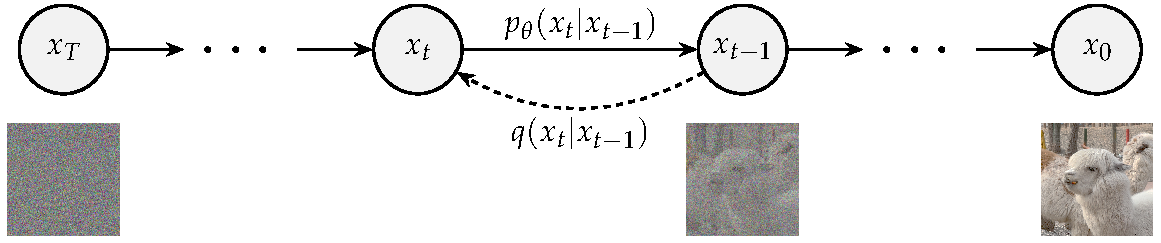
\includegraphics[width=0.9\textwidth]{figures/Markov-chain/DDPM.pdf}
    \caption{DDPM示意图}\label{fig:DDPM}
\end{figure}

DDPM中的Markov核都是Gauss分布,具体如下:
\begin{itemize}
    \item 扩散过程:假设真实图片的分布是$q(x_0)$,这就应该$x_0$的初始分布. 扩散过程从$x_{t-1}$到$x_t$就是在$x_{t-1}$上加上一个小的Gauss噪声扰动,因此我们可以写出它的转移核和初始分布:
    \[q(x_t|x_{t-1}) := \mathcal{N}(x_t; \sqrt{1 - \beta_t x_{t-1}}, \beta_t \mathbf{I}),\quad x_0\sim q(x_0).\]
    这里$\beta_t$是一个超参数,$\mathcal{N}(x;\mu,\Sigma)$是Gauss分布$\mathcal{N}(\mu,\Sigma)$在点$x$的概率密度. 
    \item 逆向过程:扩散的末端$x_T$是一个完全的Gauss噪声,我们不妨设它是标准Gauss分布,即$x_T\sim\mathcal{N}(0,\mathbf{I})$. 逆向过程希望从$x_t$恢复到$x_{t-1}$,因此我们应该用$x_t$和$t$来预测$x_{t-1}$的期望,我们用一个神经网络$\mu_\theta(x_t,t)$来表示这个期望. 于是,逆向过程的转移核和初始分布为:
    \[
    p_{\theta}(x_{t-1}|x_t) := \mathcal{N}(x_{t-1}; \mu_{\theta}(x_t, t), \sigma_t^2\mathbf{I}),\quad p(x_T)=\mathcal{N}(x_T;\mathbf{0},\mathbf{I}).
    \]  
    这里$\sigma_t$是一个超参数. 
\end{itemize}

根据我们的上面的讨论,扩散模型有两个任务:

\begin{enumerate}
    \item 训练一个逆向过程,使得$p_\theta(x_0)$尽可能接近数据的分布$q(x_0)$. 
    \item 采样一个逆向过程,对一个训练好的扩散模型,这个步骤可以从噪声$x_T$出发生成一张有结构的图片$x_0$. 
\end{enumerate}

对于第一步,我们需要将训练的损失函数写出. 对于第二步,我们需要一个采样的方法. 由于采样比训练更简单,而且训练依赖采样,所以我们会先讨论采样. 

\subsection{采样逆向过程}

因为逆向过程是一个Markov链,我们需要能够采样一个Markov链的状态序列. 因为随机变量之间有相互依赖关系,Markov链的采样不是那么平凡的. 但是,Markov性给了我们一种采样的方法. 

考虑Markov链$X_k$,转移核为$p(i,j)$,初始分布为$\lambda$. 我们可以通过以下方法采样$X_k$:
\begin{enumerate}
    \item 从初始分布$\lambda$采样$X_0$.
    \item 对于$k=1,2,\dots$,从$p(X_{k-1},\cdot)$采样$X_k$.
\end{enumerate}
根据Markov性,在给定$X_{k-1}$的情况下,$X_k$的分布只依赖于$X_{k-1}$,所以这一采样方法可以正确地采样$X_k$. 根据这一原则,我们可以很具体地将逆向过程的采样算法写出. 

\begin{enumerate}
    \item $x_T \sim \mathcal{N}(0, \mathbf{I})$
    \item 对 $t = T, \ldots, 1$,重复以下步骤采样$x_{t-1}$:
    \begin{enumerate}
        \item 如果 $t\geq 1$,采样$z \sim \mathcal{N}(0, \mathbf{I})$;否则,$z = 0$.
        \item $x_{t-1} = \mu_\theta(x_t,t) + \sigma_t z$.
    \end{enumerate}
    \item 输出$x_0$.
\end{enumerate}

为了和后面训练部分对应,我们需要将2.(2)中的步骤重写为另一个等价的形式,现在可以先不管为什么要这么做. 令$\alpha_t=1-\beta_t$,$\bar\alpha_t=\prod_{s=1}^t\alpha_t$,$\epsilon_\theta(x_t, t)$是$\mu_\theta(x_t,t)$的重参数化:
\[
\mu_{\theta}(x_t, t) =  \frac{1}{\sqrt{\alpha_t}} \left( x_t - \frac{1-\alpha_t}{\sqrt{1 - \bar{\alpha}_t}}\epsilon_{\theta}(x_t, t) \right).
\]
于是,我们可以将2.(2)重写为:
\[x_{t-1} = \frac{1}{\sqrt{\alpha_t}} \left( x_t - \frac{1-\alpha_t}{\sqrt{1-\bar\alpha_t}} \epsilon_\theta(x_t, t) \right) + \sigma_t z.\]


\subsection{训练逆向过程}

接下来我们讨论训练逆向过程的损失函数. 我们需要衡量$p(x_0)$和$q(x_0)$的差异,一个常用的选择是\emph{交叉熵},我们将会在下一章中详细讨论这一概念. 此时,我们先接受交叉熵的概念,将损失函数写为:
\[
\E_q[-\log p_\theta(x_0)]=-\int q(x_0)\log p_\theta(x_0)\d x_0.
\]

为计算这一表达式,我们需要将$p_\theta(x_0)$的表达式算出. 类似HMM,我们用$x_{i:j}$表示$x_i,\dots,x_j$. 

根据全概率公式:
\[
    \begin{aligned}
        p_\theta\left(x_{0}\right)&=\int  p_\theta\left(x_{0:T}\right) \d  x_{1:T}\\
            &= \int p_\theta\left(x_{0:T}\right) \frac{q\left(x_{1:T} | x_{0}\right)}{q\left(x_{1:T} | x_{0}\right)} \d  x_{1:T} \\
        &= \int q\left(x_{1:T} | x_{0}\right) \frac{p_\theta\left(x_{0:T}\right)}{q\left(x_{1:T} | x_{0}\right)} \d  x_{1:T} \\
        &= \int q\left(x_{1:T} | x_{0}\right) p_\theta\left(x_{T}\right) \prod_{t=1}^T \frac{p_\theta\left(x_{t-1} | x_{t}\right)}{q\left(x_{t} | x_{t-1}\right)}\d  x_{1:T}.
    \end{aligned}    
\]

接下来,我们计算并放缩损失函数,最终得到容易利用梯度进行优化\footnote{对于优化相关的详细讨论,见\Cref{part:decision-optimization}. }
    的形式:
\[
\begin{aligned}
    K & =-\int q\left(x_{0}\right) \log p\left(x_{0}\right) \d x_{0} \\
    & =-\int q\left(x_{0}\right) \cdot \log \left[\int q\left(x_{1:T} | x_{0}\right) \cdot p\left(x_{T}\right) \prod_{t=1}^T \frac{p\left(x_{t-1} | x_{t}\right)}{q\left(x_{t} | x_{t-1}\right)}\d x_{1:T}\right]\d x_{0}.
\end{aligned}
\]
利用Jensen不等式(\Cref{thm:jensen}),$\log(\int q f\d x)\geq\int q\log(f)\d x$,这可以被放缩为:
\[
\begin{aligned}
    K \leq & -\int q\left(x_{0:T}\right) \log \left[p\left(x_{T}\right) \prod_{t=1}^T \frac{p\left(x_{t-1} | x_{t}\right)}{q\left(x_{t} | x_{t-1}\right)}\right] \d x_{0:T}:=L.
\end{aligned}
\]

可以证明(留到下章作业),$L$可以被写作:
\[
\begin{aligned}
    \E_q[&\underbrace{D_{\KL}\left(q\left(x_T | x_0\right) \| p\left(x_T\right)\right)}_{L_T}+\\
    &\sum_{t>1} \underbrace{D_{\KL}\left(q\left(x_{t-1} | x_t, x_0\right) \| p_\theta\left(x_{t-1} | x_t\right)\right)}_{L_{t-1}} \underbrace{-\log p_\theta\left(x_0 | x_1\right)}_{L_0}],
\end{aligned}
\]
其中$D_{\mathrm{KL}}(f\|g)=\int f\log(f/g)\d x$是K-L散度. 

接下来我们分别讨论每一部分的计算. 
\begin{itemize}
    \item $L_T$不含参数,所以可以丢掉. 
    \item $L_0$和输出的数据格式有关(例如图片如何编码),需要具体问题具体处理,所以这里不讨论. 
    \item 唯一需要处理的是$L_1$到$L_{T-1}$的计算. 
\end{itemize}

由于$p_\theta\left(x_{t-1}|x_t\right)=\mathcal{N}\left(x_{t-1} ; \mu_\theta\left(x_t, t\right), \sigma_t^2 \mathbf{I}\right)$,可以算得(见习题\lhysays{出一下}):
\[
L_{t-1}=\E_q\left[\frac{1}{2 \sigma_t^2}\norm{\tilde{\mu}_t\left(x_t, x_0\right)-\mu_\theta\left(x_t, t\right)}^2\right]+C,
\]
其中$C$是一个不含$\theta$的常数,并且
\[
\tilde{\mu}_t\left(x_t, x_0\right):=\frac{\sqrt{\bar{\alpha}_{t-1}} \beta_t}{1-\bar{\alpha}_t} x_0+\frac{\sqrt{\alpha_t}\left(1-\bar{\alpha}_{t-1}\right)}{1-\bar{\alpha}_t} x_t.
\]

因为$C$是一个常数,我们可以丢弃它而不影响最优值. 接着,利用重参数化
\[
\mu_{\theta}(x_t, t) =  \frac{1}{\sqrt{\alpha_t}} \left( x_t - \frac{1-\alpha_t}{\sqrt{1 - \bar{\alpha}_t}}\epsilon_{\theta}(x_t, t) \right),
\]
引入随机变量$\epsilon\sim\mathcal{N}(0,\mathbf{I})$,我们可以将$L_{t-1}$写作:
\[
\E_{x_0, \epsilon}\left[\frac{\beta_t^2}{2 \sigma_t^2 \alpha_t\left(1-\bar{\alpha}_t\right)}\norm{\epsilon-\epsilon_\theta\left(\sqrt{\bar{\alpha}_t} x_0+\sqrt{1-\bar{\alpha}_t} \epsilon, t\right)}^2\right].
\]

如果我们想用基于梯度方法对它进行优化,我们需要计算它的梯度. 然而,这是一个期望,没有办法直接求梯度,所以我们用采样到的$x_0$和$\epsilon$代替期望中的$x_0$和$\epsilon$,把它当成期望来求梯度. 

另外,如果把所有$L_{t-1}$都用来训练,当总时长$T$非常大的时候,训练也会非常困难,所以在实际训练中,我们会均匀随机选择一个$t$,对$L_{t-1}$进行优化. 

最终,我们得到了扩散模型的训练算法:

\begin{itemize}
    \item 重复以下步骤直到收敛:
    \begin{itemize}
        \item 采样$x_0 \sim q\left(x_0\right)$.
        \item 采样$t \sim \U(\{1, \ldots, T\})$.
        \item 采样$\epsilon \sim \mathcal{N}(0, \mathbf{I})$.
        \item 用下面的梯度做一次优化:
        \[
        \nabla_\theta\norm{\epsilon-\epsilon_\theta\left(\sqrt{\bar{\alpha}_t} x_0+\sqrt{1-\bar{\alpha}_t} \epsilon, t\right)}^2.
        \]
    \end{itemize}
\end{itemize}


\section{章末注记} \lhysays{TODO}

Euclid在他伟大的《几何原本》\footnote{实际上,Euclid的书名直译是“原理”,并没有“几何”一词. 这说明Euclid其实在探求某些更加本质的东西,这样的思想后来被发展为了我们今天的\emph{形式推理系统}或\emph{公理系统}.}最早尝试将数学整理为一个完整的\emph{公理系统}. 

\section{习题} \lhysays{TODO}